\section{设计结果}

\subsection{设计交付物说明}
本设计所有源文件都在mycpu(AXI接口)中,将文件add到vivado中即可综合实现上板或仿真,将文件放入CO-lab-material-CQU/mycpu文件夹中即可使用verilator/axi进行测试。

\subsection{设计演示结果}
\subsubsection{功能测试}
\begin{figure}[H]
    \centering
    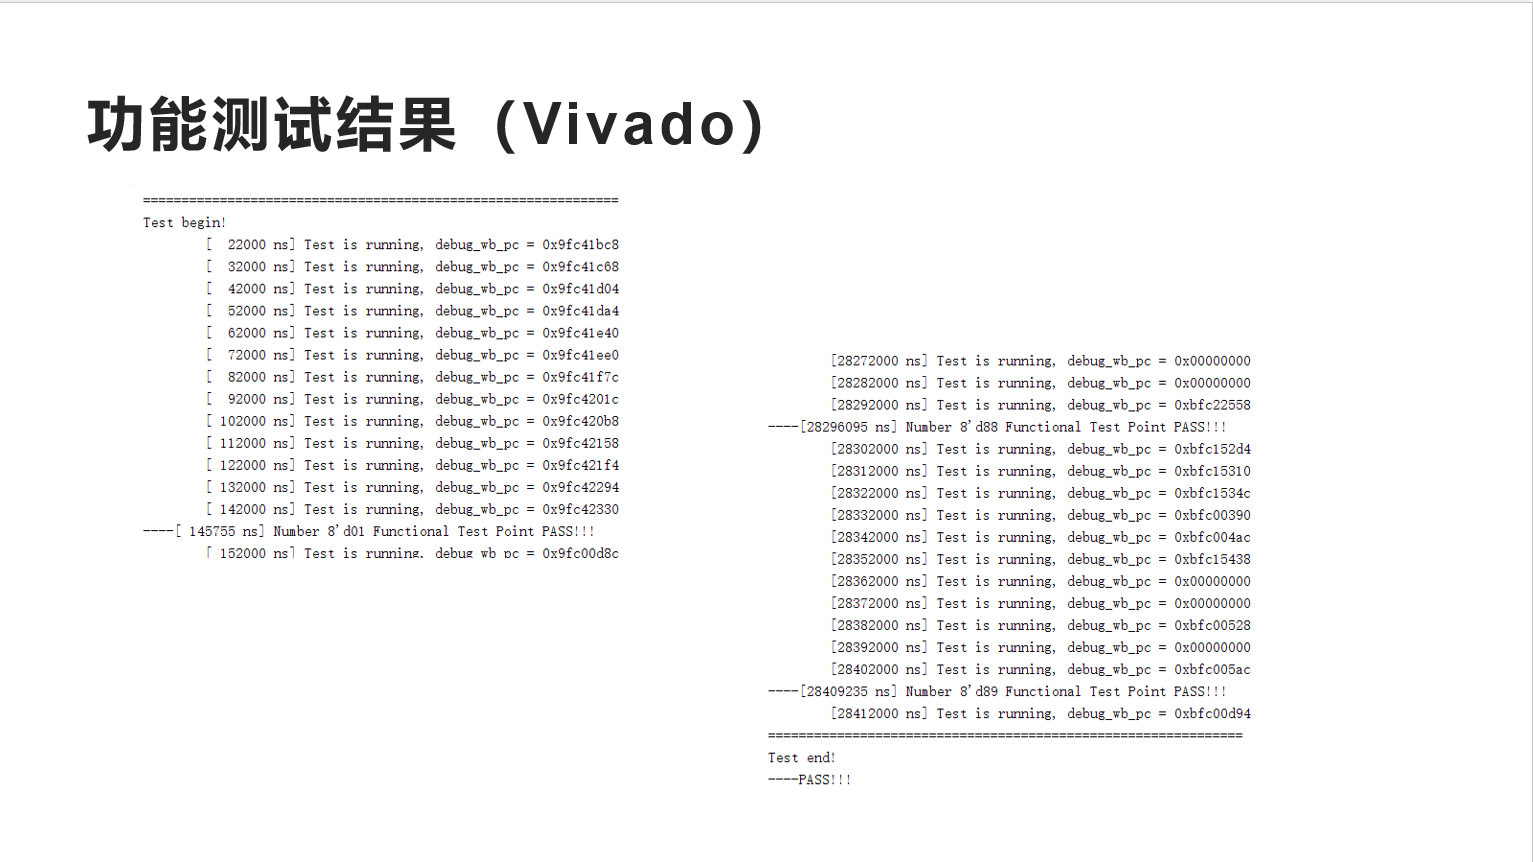
\includegraphics[width=\textwidth]{image/fun_vivado.png}
    \caption{vivado功能测试}
\end{figure}
\begin{figure}[H]
    \centering
    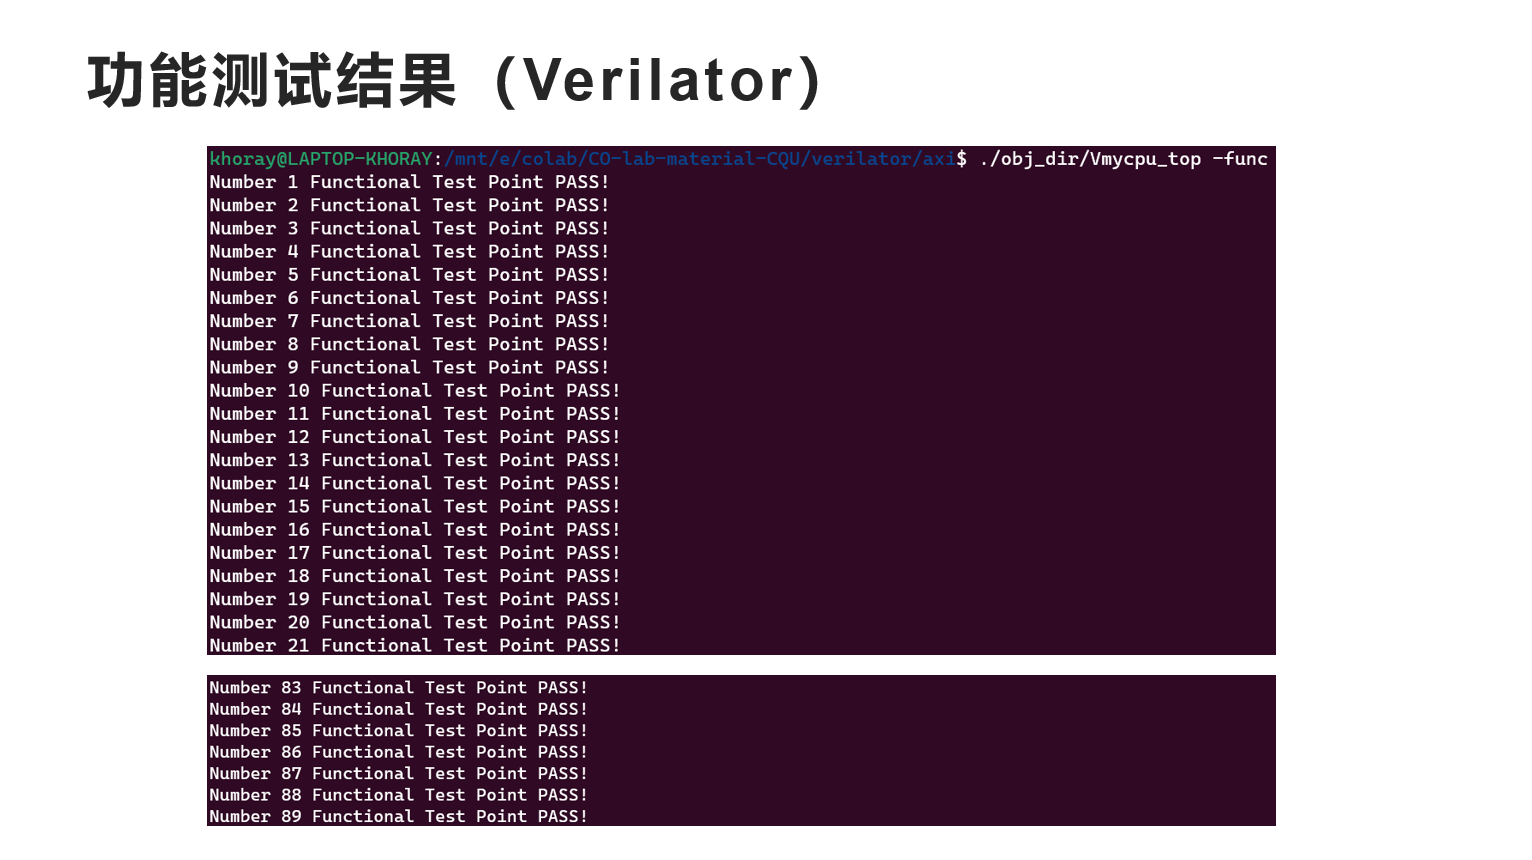
\includegraphics[width=\textwidth]{image/fun_veri.png}
    \caption{verilator功能测试}
\end{figure}

\subsubsection{性能测试}
\begin{figure}[H]
    \centering
    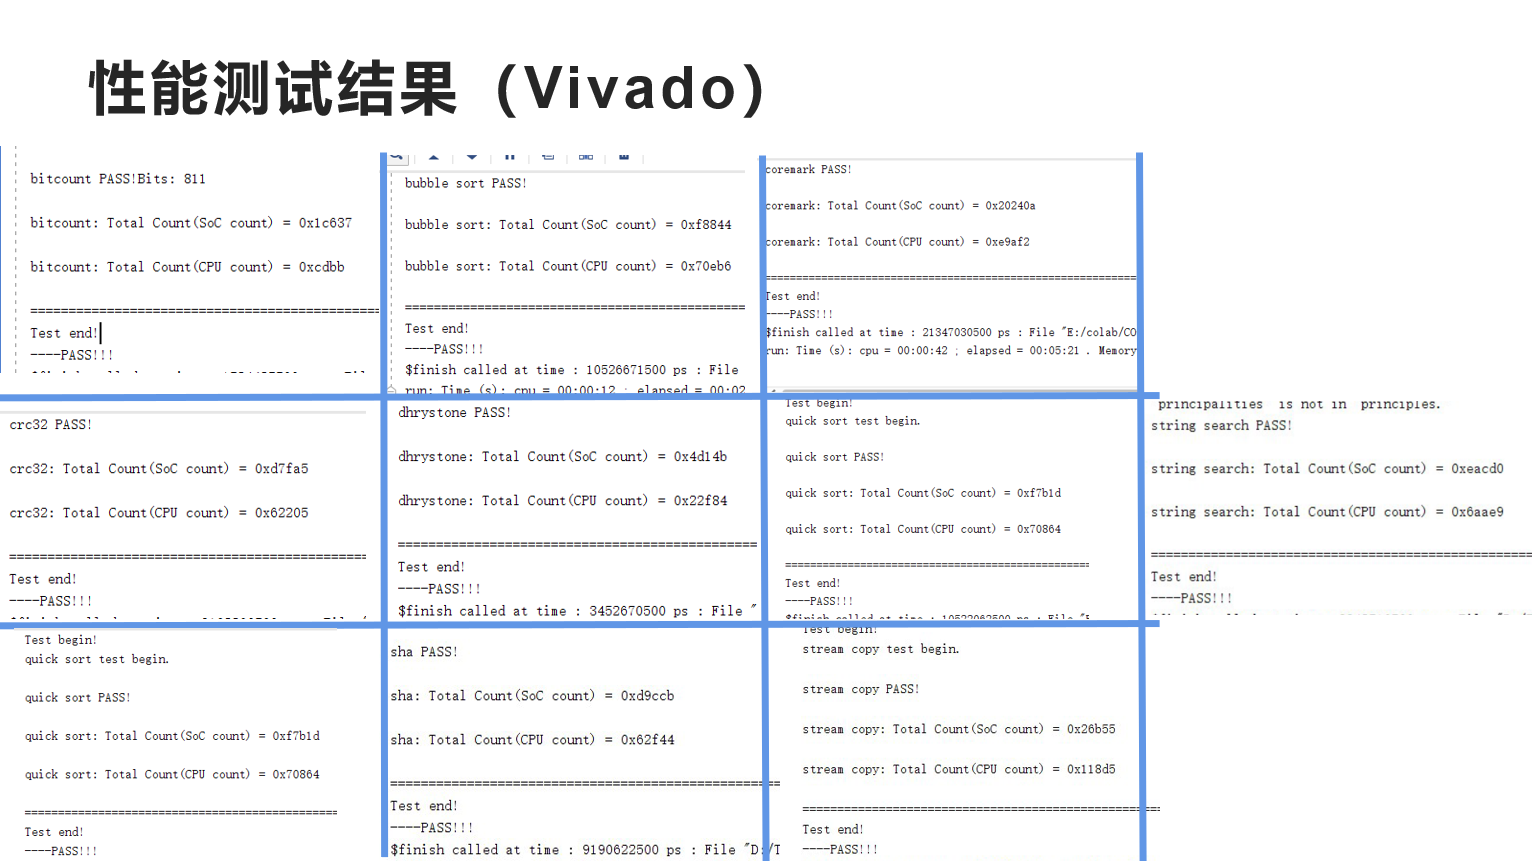
\includegraphics[width=\textwidth]{image/perf_vivado.png}
    \caption{vivado性能测试}
\end{figure}
\begin{figure}[H]
    \centering
    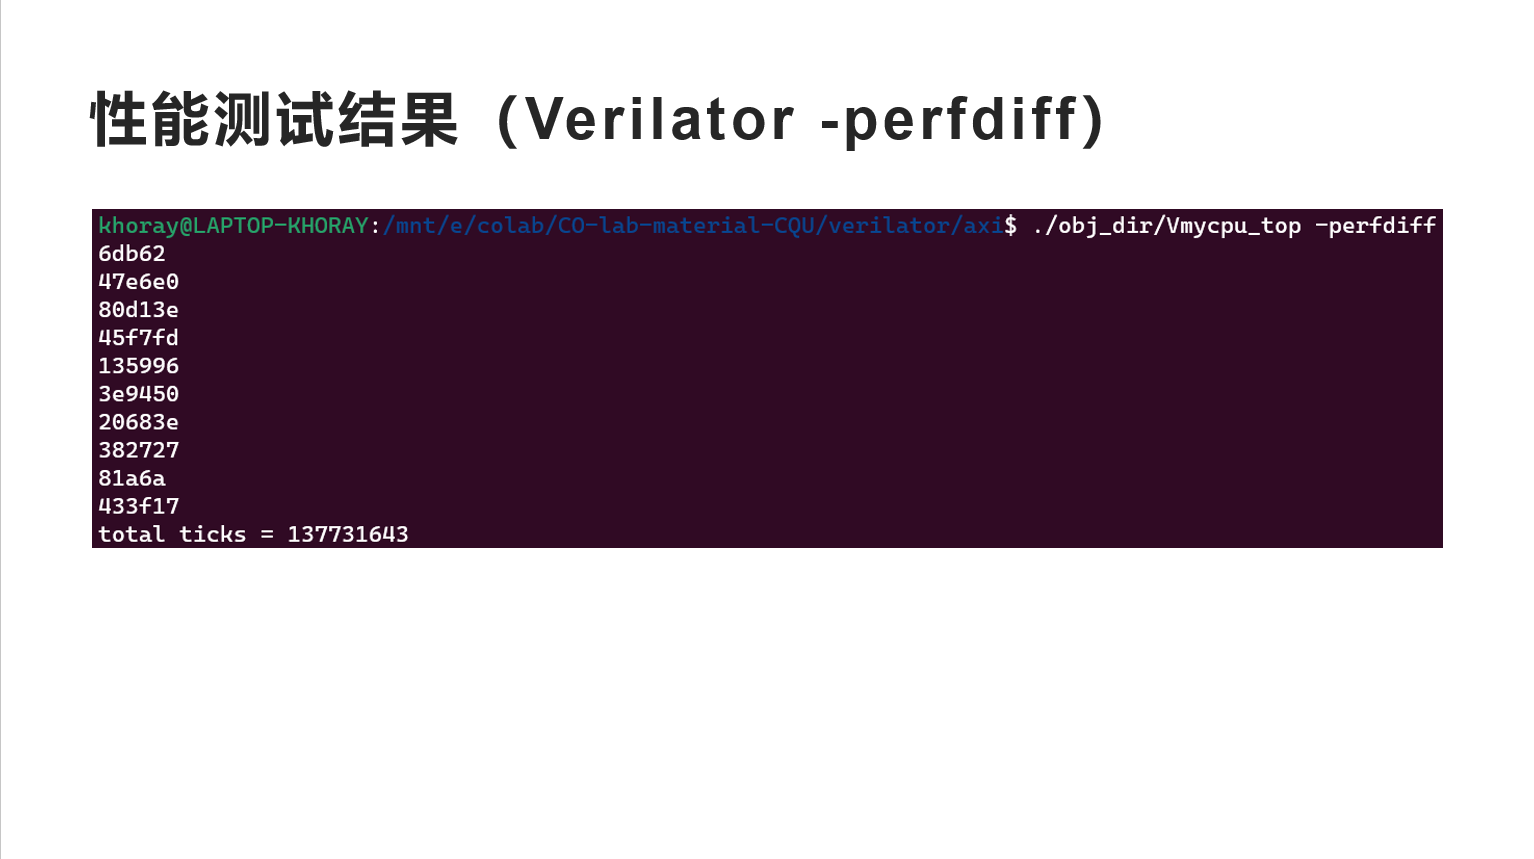
\includegraphics[width=\textwidth]{image/perf_veri.png}
    \caption{verilator性能测试}
\end{figure}
\begin{figure}[H]
    \centering
    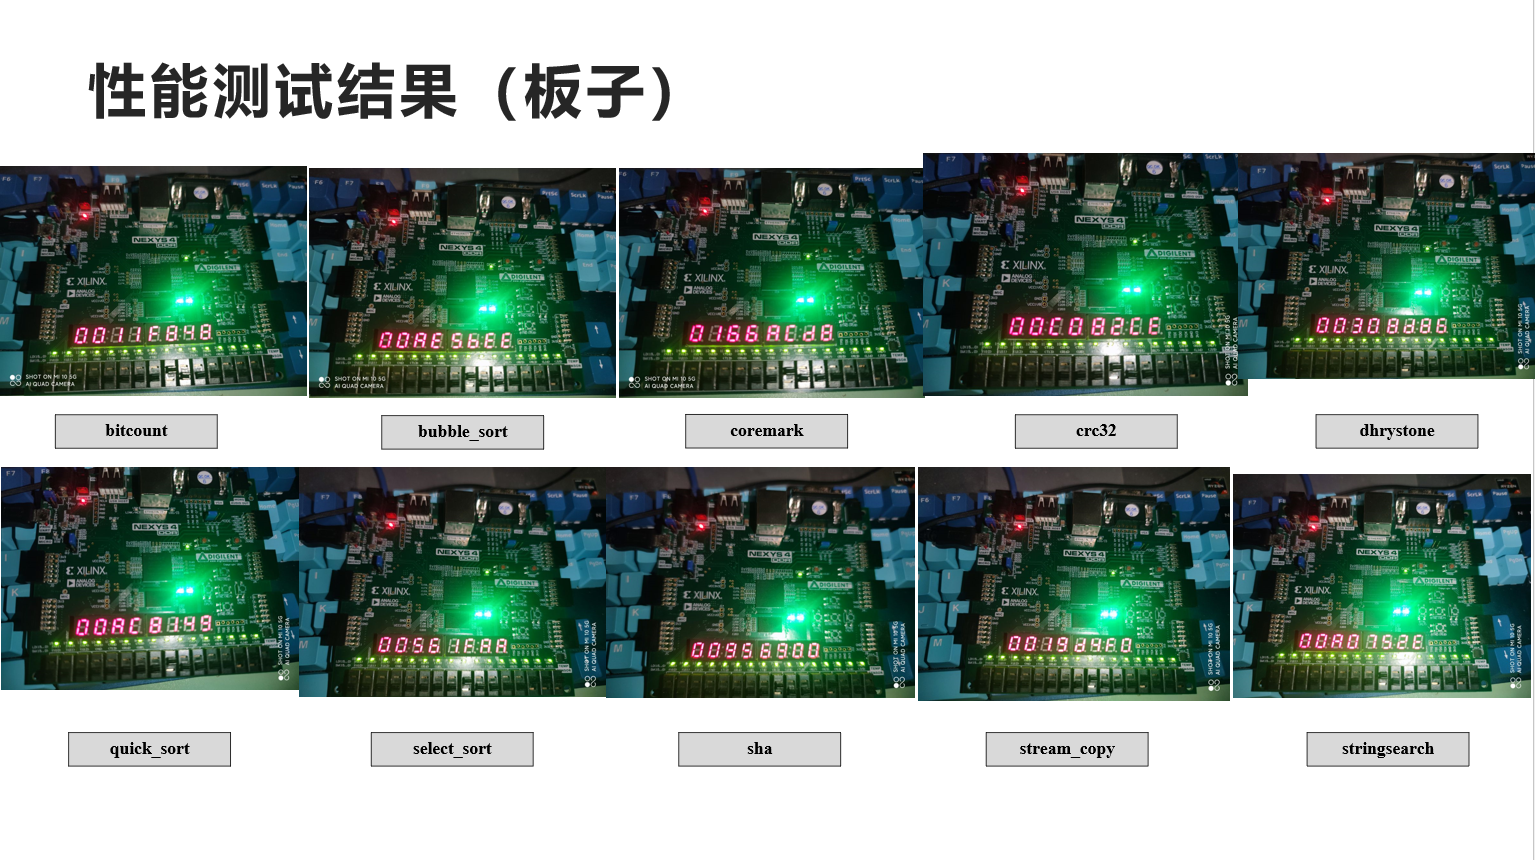
\includegraphics[width=\textwidth]{image/perf_fpga.png}
    \caption{开发板性能测试}
\end{figure}
\begin{figure}[H]
    \centering
    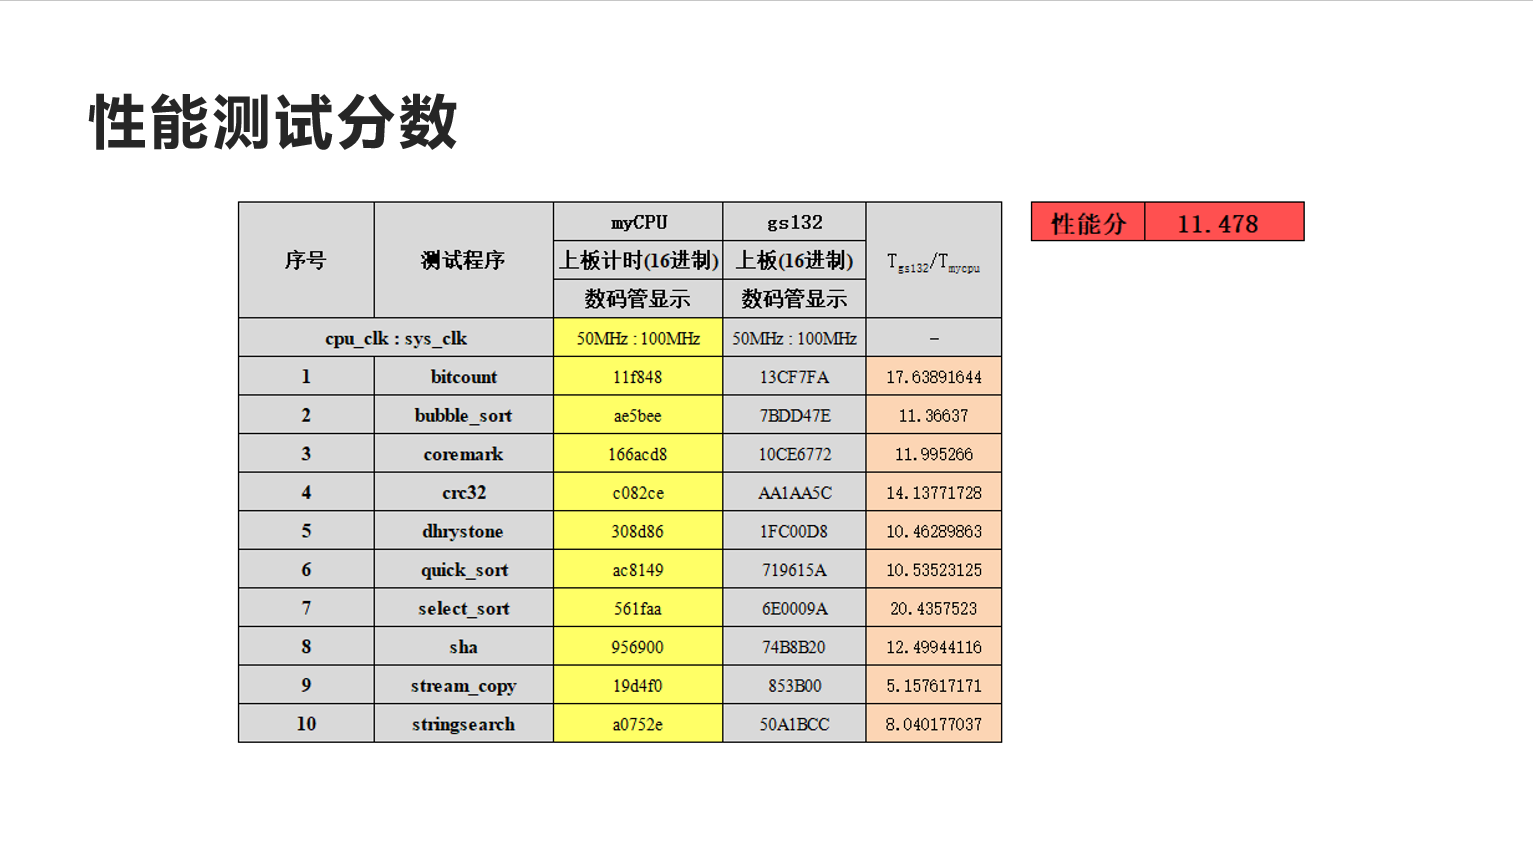
\includegraphics[width=\textwidth]{image/perf_score.png}
    \caption{性能测试分数}
\end{figure}
